\section{Nested Newton single channel flow}
\newrefsegment

%---------------------------------------------------------------------------------
\section*{Quality Assurance}
{{\footnotesize
\begin{tabular}{p{22mm-2pt}@{}p{27mm-2pt}@{}p{18mm}@{}p{27mm-2pt}@{}p{18mm}@{}p{27mm-2pt}@{}p{\textwidth-139mm-1pt}} \hline
    \rowcolor{dgrey4}
\textbf{Date} & \textbf{Author} & \textbf{Initials} & \textbf{Review} & \textbf{Initials} & \textbf{Approval} & \textbf{Initials}  \\ \hline
21 Sep 2017 & Jan Noort & & ... & & ... &   \\ \hline
  \end{tabular}
}}

%---------------------------------------------------------------------------------
\section*{Version information}
\begin{tabular}{@{}p{23mm}@{}p{0mm}p{\textwidth-23mm-30pt}}
\textbf{Date of study}    & \textbf{:} & 27 February 2019 \\
\textbf{Executable(1)}   & \textbf{:} & Deltares, D-Flow FM Version 1.1.192.51311, Sep 21 2017, 18:48:09 (c48) \\
\textbf{Location}         & \textbf{:} & \url{https://repos.deltares.nl/repos/dscTestBench/cases/e02_dflowfm/f100_1D/c04\_closed\_channel\_circle} \\ 
\textbf{SVN revision}     & \textbf{:} & TortoiseSVN 1.9.4, Build 27285 - 64 Bit
\end{tabular}

%---------------------------------------------------------------------------------
\section*{Purpose}
The purpose of this validation case is to test the Nested Newton non linear solver. 
The implementation of the Nested Newton method is described in section "Nested Newton non linear solver" of the \citet{DFLOWFM_TRM}. 
The Nested Newton method was published in \cite{Casulli2013}

%---------------------------------------------------------------------------------
\section*{Linked claims}


%---------------------------------------------------------------------------------
\section*{Approach}
Three simulations have been prepared and all the input is specified using D-Flow flexible mesh (FM). 


%---------------------------------------------------------------------------------
\section*{Conclusion} 
The result shows that pressurized flow in a closed channel is correctly solved by \DFLOWFM.

%---------------------------------------------------------------------------------
\section*{Model description}
The main setup for the testcases is a straight channel of approximately 1800 meters and with 20 computational points. 
The roughness is set to a Chezy value of 45 $m^{1/2}s^{-1}$. 
Upstream a water level boundary is set to 1.5 m and downstream the water level boundary condition is set to 0.1. 
The model is started with an initial water level of 0 m (= dry system).
Furthermore for comparison sake an extra Preismann slot is added to the model of 0.001 m.

The cross section of the models are different.
\begin{itemize}
	\item In c04\_closed\_channel\_circle a circular cross section with a diameter of 0.16 m is used. 
	\item In c05\_closed\_channel\_rectangle a rectangular cross section of 0.2 x 0.2 is used. 
	\item In c06\_closed\_channel\_egg an egg type cross section with a diameter of 0.16 m is used. 
\end{itemize}


%---------------------------------------------------------------------------------
\section*{Results}
The results of D-FlowFM are compared to the results from SOBEK3. 
The main difference in water level occurs at chainage 1628 m from the upstream boundary.


\begin{figure}[H]
	\begin{center}
		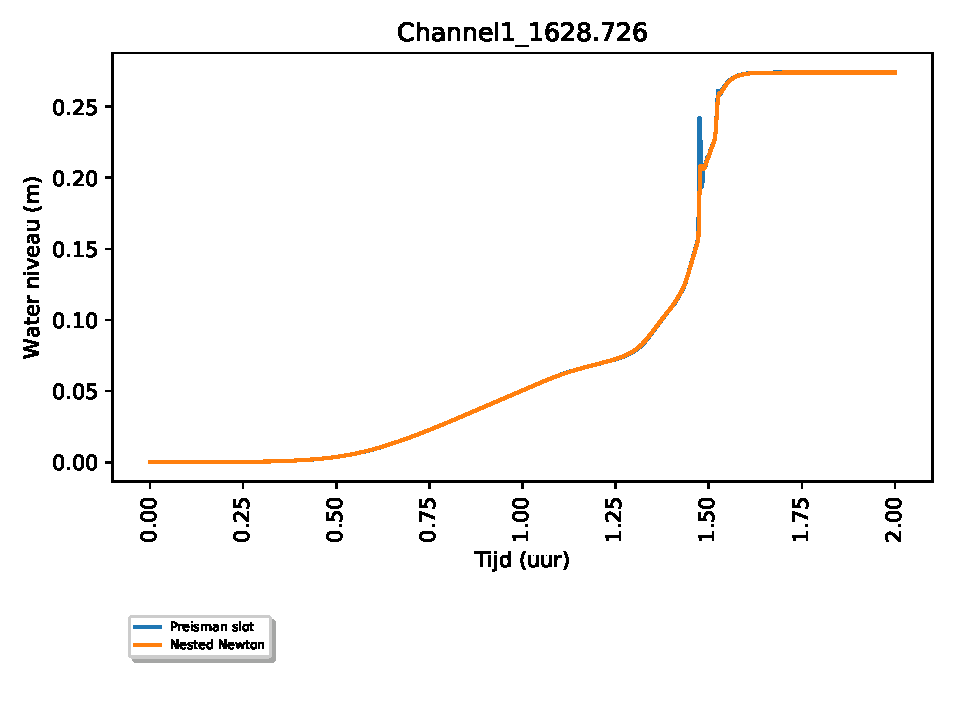
\includegraphics[width=0.7\columnwidth]{figures/diff_verschil_circular.pdf}
	\end{center}\caption{Comparison of SOBEK results to \DFLOWFM results for a circular shaped cross section}
	\label{fig:NNcircle}
\end{figure}
\begin{figure}[H]
	\begin{center}
		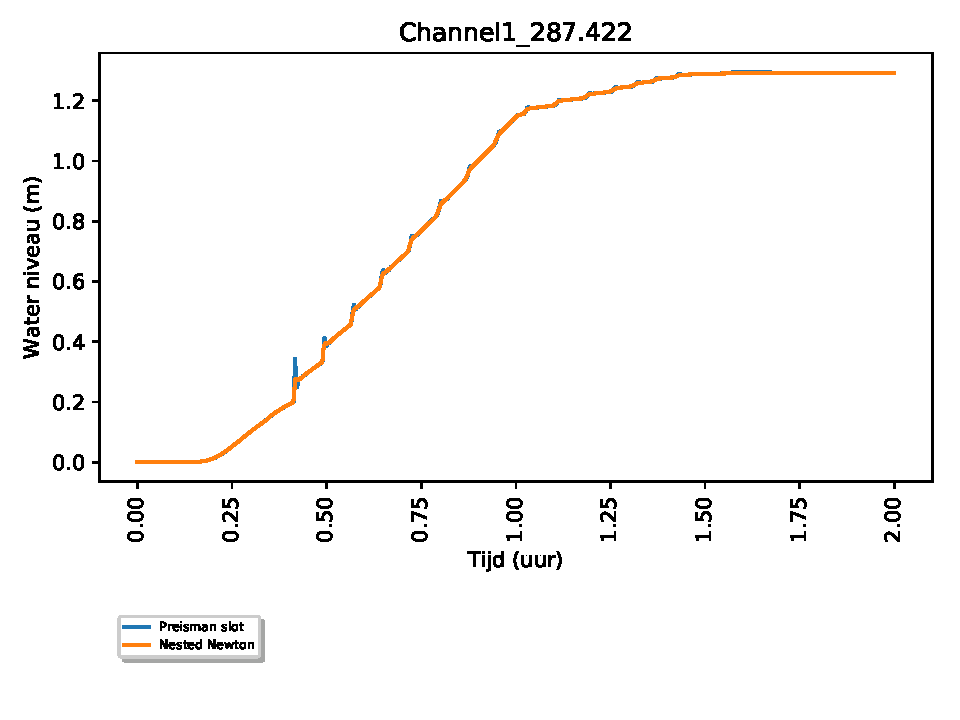
\includegraphics[width=0.7\columnwidth]{figures/diff_verschil_rectangular.pdf}
	\end{center}\caption{Comparison of SOBEK results to \DFLOWFM results for a rectangular shaped cross section}
	\label{fig:NNrectangle}
\end{figure}
\begin{figure}[H]
	\begin{center}
		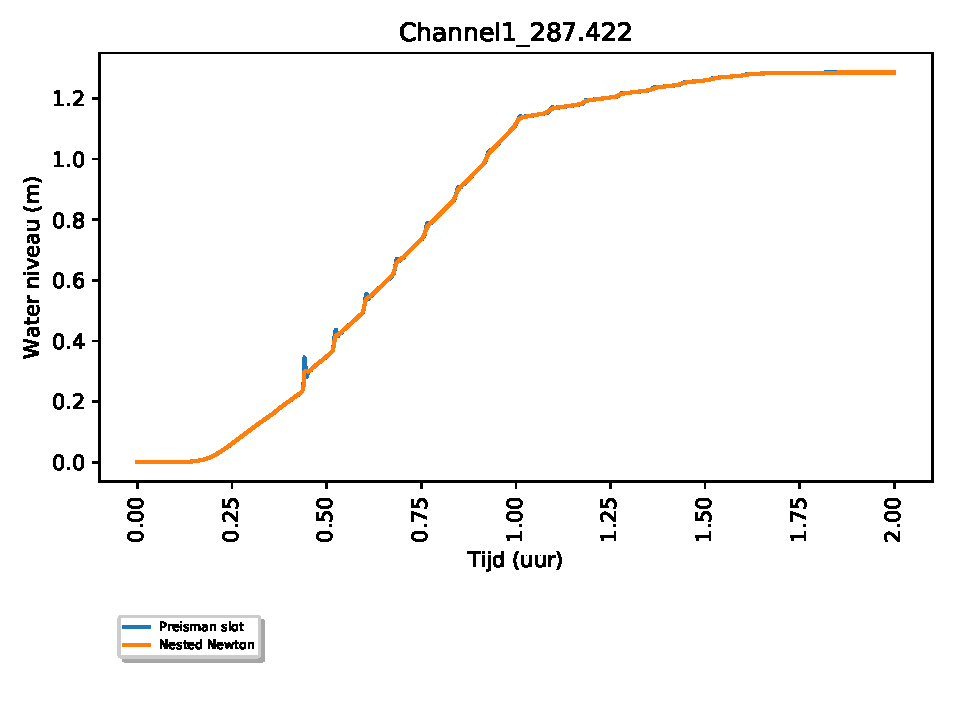
\includegraphics[width=0.7\columnwidth]{figures/diff_verschil_egg.pdf}
	\end{center}\caption{Comparison of SOBEK results to \DFLOWFM results for an egg shaped cross section}
	\label{fig:NNegg}
\end{figure}

The main difference between the two models is the spikes that occur in SOBEK3 and that are less prominent in \DFLOWFM.

The effect of the Preisman slot is presented in figure \ref{fig:NNslot}
\begin{figure}[H]
	\begin{center}
		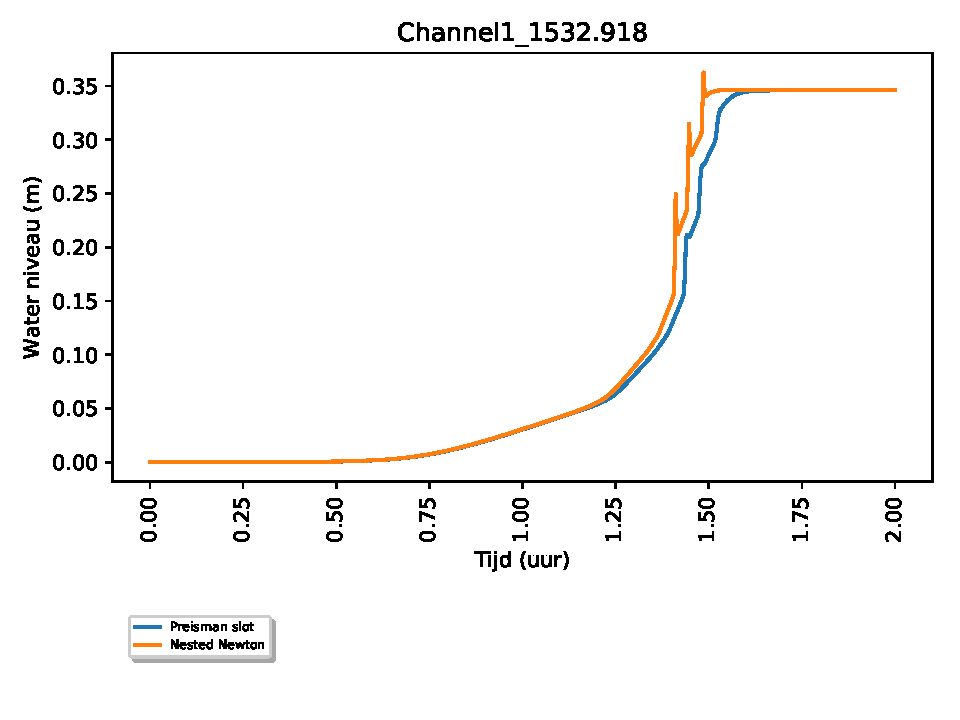
\includegraphics[width=0.7\columnwidth]{figures/diff_verschil_circular_w_0.pdf}
	\end{center}\caption{Comparison of \DFLOWFM results for a circular shaped cross section with Preisman slot resp equal to 0.001 and 0.0}
	\label{fig:NNslot}
\end{figure}
%---------------------------------------------------------------------------------
\section*{Analysis of results}
The result shows that the water level and the bed level behavior of both models (structures and unstructured grids) are almost the same and comparable to Delft3D. The new version (executable(1)) performs well with unstructured grid and more stable at the upstream boundary.

%---------------------------------------------------------------------------------
\printrefsegment
